\documentclass[
    11pt,
	% colorful,
	% boxey,
]{tufte-style-thesis}

%	package inclusions for this specific documentation file. the .cls does not neet them.
\usepackage{lipsum}		% the chad package
\usepackage{textgreek}	% for greek
\usepackage{imakeidx}	% for index
\usepackage{multicol}
\makeindex[columns=3]

\addbibresource{refs.bib} % for biblatex

% INFO : used in the titlepage, copyright and stuff.
\author{Sylvain Kern}
\title{\texttt{tufte-style-thesis},\\a Tufte-styled \LaTeX{} class for theses}
\subtitle{Actually more of a mix\\between Edward Tufte and Robert Bringhurst}
\university{A fancy University}
\lab{An even fancier Lab}
\person{Supervisor}{their name}{their job}
\person{Cosupervisor}{also their name}{also their job}
\person{Jury members}{jury 1}{jobs}
\person{}{jury 2}{\dots}
\logo{example-image-a}
\logo{example-image-b}
\logo{example-image-c}
\shoutouts{For my homies}

\begin{document}

\maketitle

\frontmatter

\chapter{Abstract}
Basically a thesis (book?) class for Tufte lovers like myself. I am aware that \texttt{tufte-latex} already exists but I just wanted to create my own thing.


\chapter{Acknowledgements}
Gabriel the king. All the \href{https://tex.stackexchange.com/}{\TeX.SE} team for answering my stupid questions.

\tableofcontents
\listoffigures
\listoftables
\listoflistings


\mainmatter

\chapter{Notes on the design}

This class is my personal mix of different book design influences: mainly the works of Edward R. Tufte,\sidecite{TufteTvdq, TufteBE, TufteEI, TufteVE}\index{Tufte, Edward R.} known for the big margin and the plentiness of sidenotes and sidecaptions. The margins are however not as prominent as in Tufte's works, the main text takes a bit more space, more like in Robert Bringhurt's typographer's bible.\sidecite{BringhurstEoTS}\index{Bringhurst, Robert} So it is a bit of a mix of Tufte and Bringhurst, with some of my own choices for other design features, as we will see through this chapter.

\section{Document layout}

While \texttt{tufte-style-thesis} is a class for typesetting theses, the general layout is pretty much the same as in a regular book. A book is traditionally divided into three major sections: the front matter, the main matter and the back matter.

The \textit{front matter}\index{front matter} is for all the stuff that comes before the main content: the preface, the acknowledgements, table of contents (\textsc{toc}) and list of various types. The pages are most widely printed in roman numerals for this part. However, I personally find it confusing and a bit useless so the page numbering system is simplified for the whole book: arabic numerals starting from the very first page of the document.\sidenote{Tufte and Bringhurst do full arabic in their work too, so I consider it legit.} The frontmatter still remains relevant because chapters are unnumbered, and \LaTeX{} conveniently places them in the \textsc{toc}.

The \textit{main matter}\index{main matter} is, as its name suggests, for the main content. Here everything is normal, arabic page numbering, normally numbered chapters. At the end of the mainmatter there are usually appendices, especially for scientific and technical textbooks ; for me, an appendix seems necessary in a thesis to put big figures, tables, and content that can be referred to in the main text but are too intrusive to put in the heart of the document. Chapters in the appendix are numbered with a letter to distinguish them from the main content. The main matter can also be cut in a couple of parts.\sidenote{I like, for instance, to put the appendix in a dedicated part.}

The \textit{back matter}\index{back matter} is the end of the book, usually for the references part and index or glossary. Chapter numbering is turned off. At the very end, a colophon\sidecite{CarterABC} can be put to state information about the printer, publisher and stuff like that.

To sum this up, the structure of a document typeset with \texttt{tufte-style-thesis} is something like this:
\begin{itemize}
  \item titlepage ;
  \item front matter (dedication, abstract, acknowledgements, table of contents, list of figures, \textit{etc}) ;
  \item main matter (main content organized in numbered chapters, an appendix with letter chapters) ;
  \item back matter (references, index, glossary, colophon).
\end{itemize}
This is how \LaTeX{} books work, and how I advise to structure a document using this class. All of this is under a single page numbering system, arabics starting right from the titlepage. Eventually, this is a really heavy layout, see how the first chapter of content starts at page 18. So do not use this class unless you have a hefty content to fit all these organizing features.


\section{Page layout}

Maybe the most distinctive aspect of this class is its page layout with its big margin to put sidenotes and captions. However this is not original at all: plenty\sidenote{\texttt{tufte-latex}:\\\noindent\url{https://www.ctan.org/pkg/tufte-latex},\\\texttt{classicthesis}:\\\noindent\url{https://www.ctan.org/pkg/classicthesis}, \dots} of other \LaTeX{} classes for books and theses do it just like me, and almost always better\sidenote{Or in a way cleaner \LaTeX{}.} I just wanted to do my own thing here, mixing what I personally like the most in these layout types, to better learn \LaTeX{} and to really internalize this kind of design. At the end of the day it may be a more Bringhursty than Tuftey kind of look, but hey, I won't change the name of this whole thing now.

So, as you might have started to notice, the main feature of this thing is the margin, with the sidenotes\index{sidenotes}, side references, and as you will discover, side captions and everything. It has three main advantages for me:\sidenote{These advantages can be seen as drawbacks for others: less space for the actually important content, irregular and somewhat unconventional design which can be harder to handle.}
\begin{itemize}
  \item it makes the main text area narrower, therefore easier to read as the line changes become smoother, sidenotes are also friendlier than footnotes ;
  \item it makes the design breathe with plenty of potential white space (when the margins are not too crowded) ;
  \item it organizes the content: non-prosaic elements are on the side, separated from the main text area which becomes less cluttered.
\end{itemize}
So this is more intended for people who like "flavoured" text: people who likes notes, parentheses, asides, \textit{etc}. It is also more suited for topics needing lots of pictures, tables, and diagrams: a novel would look terrible with this kind of layout.

Another small detail on the sidenotes, the flag of a note is in superscript in the text, but the note itself is introduced by a number in full size: this is in superscript \dots\sidenote{\dots whereas this is in normal size.} This is again one of Bringhurst's advices.


\section{Headers, lists, and other content-organizing features}

The principle here is to give structuring elements which are as unobtrusive as possible, while remaining clear and easy to follow. For example, the bold headers of vanilla \LaTeX{} have been changed for more subtle italic ones. Chapters titles have been simplified to their essential parts --a number and a title-- and put as high as possible: it is completely useless to me to start a new chapter at the middle of a page.\sidenote{Bringhurst roasts this kind of chapters in his \textit{Elements}: \textit{"In modern books, where the titles are shorter and the margins have been eaten by inflationary pressure, a third of the page somewhat lies vacant just to celebrate the fact that the chapter begins"}.} Though, some of space is left after the title to let it breathe a little bit ; this is a feature of Tufte's books.

The \textsc{toc}, and the other lists as well as the index and references section are thought to be that way: friendly and unobtrusive. For example, in the \textsc{toc}, the traditional dotted lines between a heading and its corresponding folio\sidenote{Just flexin, folio is a fancy term for saying "page number".} is useless and unfriendly: why have the reader to follow a line with their eyes instead of just placing the page number next to the heading? So I adapted the \textsc{toc} to make it both expressive and light/minimalistic.\sidenote{I find Tufte- and Bringhurst-style \textsc{toc}s too empty, at least for a thesis.} It does not support deeper headings than the section, because I think nobody looks for such detail in the table of contents.


\section{Fonts and paragraph typography}

This class has three fonts.\index{fonts}

The main text is typeset with a version of Linux Libertine,\sidecite{Libertine}\index{Linux Libertine} with enhanced math support. Here it is in \textbf{bold} and \textit{italic}.

Sans serif text, like in the titlepage, part titles and page headers (not chapter/section titles, but small reminders at the very top of the pages) are in sans serif {\sffamily Gill Sans}\index{Gill Sans}, actually Gillius, a version of Gill Sans for \LaTeX{}. Here it is in {\sffamily\bfseries bold} and {\sffamily\itshape italics}. Gill Sans is a humanist sans-serif typeface, which I find both elegant and minimalistic. It is less harsh than grotesk fonts like Helvetica or Arial.

Mono text, for code listings, is \texttt{Droid Sans Mono}\index{Droid Sans Mono}. It is smoother to my taste than the default courier-like font. Here it is in {\ttfamily\itshape italics} (unfortunately it does not support bold --yet).

The prose is organized in paragraphs indented at the first line, as it is classically seen. The first paragraph that comes after a heading, however, is not indented.\sidenote{It is again an advice from Bringhurst: \textit{"The simplest way to start any block of prose is to start from the margin, flush left [\dots]."}} The text is by default not justified on the right like in Tufte's books. Apparently it makes the lines easier to recognize and follow with the eyes ; I do not find this irregularity unpleasing. But \textit{do not worry}, it can be fully justfied really easily.\sidenote{I hope people have not been bummed out at by not seeing the right-justfication.}

\bgroup\justifying
For true microtypography\index{microtypography}, when the text is fully justified (like this one), the dashes, commas, points and other stuff slightly protrude in the margin to make it seem more justified than it really is.\sidenote{Paradoxically, it seems more justified than when it is truly justified. See by yourself: put a ruler (or the side of the window on the right side of the text and see how the comma slightly protrudes).} For flush left text, the typesetting algorithm has also been upgraded from standard \LaTeX, reducing the line length and space width variance, and hyphenating as less as possible. Also, the spaces between small caps increase a little bit, as well as they can be increased for full caps text.
\egroup


\section{Ideas behind the design}

\index{design}These are just some thoughts I gathered that I find interesting to consider when making designs, closely or remotely.

As Antoine de Saint-Exupéry\index{de Saint-Exupéry, Antoine} once wrote:\sidecite{StExupery} \textit{"Perfection has been reached not when there is nothing left to add, but when there is nothing left to take away"}. To me, this means that minimalism is a key aspect of document design. The features and the layout must let the true content express itself: a good typography is completely transparent. That is why the design is dependent of the content: a novel and a math textbook will have completely different designs.

However, this whole Tufte-style design is far from transparent. It is easily recognizable, and people will notice the somewhat unusual design statements. Paul Rand\index{Rand, Paul} said,\sidenote{Yeah, I lazily picked the two citations on the first page of the tufte-style book class showcase. Though, I find Paul Rand's a bit condescending, like, \textit{"people know nothing about good design"}.} \textit{"The public is more familiar with bad design than good design. It is in effect, conditioned to prefer bad design, because that is what it lives with. The new becomes threatening, the old reassuring"}. Edgar Tufte completely re-thought the way to display scatterplots, curves and axes, boxplots and histograms, but most people are not used to see this optimized representation, so is it a better design if most people have to give some extra effort to adapt to it ?

Then, good design must be a cultural thing. To aim perfection, one must make a blend between innovation and tradition, to be percieved as smooth as possible for the majority of people.

So, yeah, I really don't know what to think. I find --actually I hope that sidenotes and margins benefit to the reading comfort instead of ruinig it. It makes more sense when there are figures, tables and heavier stuff, but hopefully it remains relevant for prose with notes.


\part{This is a part}

\chapter{Using this class}

\section{Dependencies}

Here are the packages already loaded, so there is no need to re-include them in your document:

\begin{wide}\setstretch{1.0}
\begin{multicols}{4}
\begin{itemize}
\item\texttt{geometry}
\item\texttt{emptypage}
\item\texttt{fullwidth}
\item\texttt{sidenotes}
\item\texttt{caption}
\item\texttt{fontenc}
\item\texttt{libertinus}
\item\texttt{libertinust1math}
\item\texttt{gillius}
\item\texttt{droidsansmono}
\item\texttt{ragged2e}
\item\texttt{titlesec}
\item\texttt{titletoc}
\item\texttt{tocloft}
\item\texttt{fancyhdr}
\item\texttt{graphicx} \item\texttt{microtype} \item\texttt{amsfonts} \item\texttt{amsmath} \item\texttt{mathtools} \item\texttt{physics} \item\texttt{xcolor} \item\texttt{mdframed} \item\texttt{tabularx} \item\texttt{booktabs} \item\texttt{enumitem} \item\texttt{hyperref} \item\texttt{etoolbox} \item\texttt{changepage} \item\texttt{placeins} \item\texttt{xparse} \item\texttt{xpatch} \item\texttt{biblatex} \item\texttt{listings}
\end{itemize}
\end{multicols}
\end{wide}

\section{The big margin}

There is a big margin, so feel free to use it as much as possible!\sidenote{Actually to your needs, if you do not have a natural usage of notes, maybe do not use this class.\\By the way, see how sidenote numbers reset on new chapters: we're back on number 1!} This chapter will cover the usage of sidenotes, side references, and other ways to use the margin.\sidenote{For float captions, see chapter \ref{chp:floats}.}

The general layout is done using the \texttt{geometry}\sidecite{pkgGeometry} package, and all the margin stuff relies on the \texttt{sidenotes}\sidecite{pkgSidenotes} package, so check its documentation:

\centering\url{http://www.ctan.org/pkg/sidenotes}\\
\RaggedRight\noindent for more in-depth information.

\subsection{Sidenotes}

To put a sidenote in the margin, use
\begin{codebox}{tex}
\sidenote[<number>][<offset>]{<sidenote text>}
\end{codebox}
\begin{itemize}
\item
\inlinecode{tex}{<number>} is an optional parameter for the sidenote number. For example, \inlinecode{tex}_\sidenote[29100][]{The sidenote.}_ does this.\sidenote[29100][]{The sidenote.}
\item
\inlinecode{tex}{<offset>} is an offset length (in pt, px, en, em\dots) to vertically offset the sidenote. A positive value will have it go down, a negative go up.
\end{itemize}

\LaTeX{} natively allows to put unformatted content in the margin with the command \inlinecode{tex}_\marginpar{<your content>}_,\marginpar{This is unformatted margin text, in fullsize.} but I advise not to use it, as it puts raw fullsize text in the margin, and does not blend well with the overall design. Instead, use\sidetext{This is just some unnumbered piece of text in the margin, but with the formatting done right.}
\begin{codebox}{tex}
\sidetext{<your text>}
\end{codebox}
This will format the margin text to match the sidenotes style.


\subsection{Side references}

The margin is also handy to put bibliographic references:\sidecite{einstein1915allgemeinen} the reader can read them directly instead of going all through the document to find the right entry in the references section. But don't worry, each reference displayed in the margin is labelled with a number and appears in a dedicated bibliography section. All in all, a side reference is displayed in the margin in a shortened form, and then again in the bibliography in the full form.

To cite a paper, use
\begin{codebox}{tex}
\sidecite{<reference label>}
\end{codebox}


\section{Full width text}

\begin{wide}
It may be handy to have the text span the whole page width, like this paragraph. Use the environment \inlinecode{tex}_\begin{wide}...\end{wide}_ to do this. It should manage page breaks properly, but it is not optimal: no not use it for too long (like for ten pages), the behavior tends to go a little wild. The behavior of \inlinecode{tex}{\sidenote}, \inlinecode{tex}{\marginpar} and \inlinecode{tex}{\sidecite} is not supported in the \inlinecode{tex}{wide} environment.

Also, for floating environments, full width figures and tables will be covered in the chapter \ref{chp:floats}, so do not use the \inlinecode{tex}{wide} environments with figures or tables (actually tables are fine, but there are specific environments for them to be in full width).
\end{wide}

\section{The skeleton}

The structure of a \LaTeX{} book is as follows:
\begin{codebox}{tex}
% preamble
\begin{document}

\maketitle % titlepage

\frontmatter % unnumbered preliminary chapters
\chapter{}
\tableofcontents

\mainmatter % main content: numbered chapters
\part{part}
\chapter{content}
\chapter{content}

\appendix % letter numbered chapters
\chapter{appendix 1}
\chapter{appendix 2}

\backmatter % everything else: references, indexes, glossaries, etc.
\printbibliography
\printindex

\end{document}
\end{codebox}

\subsection{The new \texttt{\textbackslash maketitle}}

The \inlinecode{tex}_\maketitle_ macro has been slightly pimped up. It now displays a custom titlepage ---like the one on this very document, as well as a copyright tag, a dedication word and a colophon.

\section{Floats}
\label{chp:floats}

The integration of floats with the Tufte layout is handled with the \texttt{sidenotes} package, loaded with the class definition. The following paragraphs show how to basically use the macros, and for more information, see the package documentation at \url{https://www.ctan.org/pkg/sidenotes}.

\subsection{Figures}

Edward Tufte's designs are known to be really tight when it comes to including images with text. The main pet peeve I had with one-column designs is when I included a small figure in the document, it had to visually break the text and generate large unpleasing blank spaces. Also, more often than not, the text width was too much for the images, resulting in huge one-liner captions for very small figures.

The 1.5-column design fixes this by putting all captions in the margins, as well as small enough figures, which tidies the document a lot.

\textfig[1]{figures/bretagne.png}{1919 map of the Finistère in French Brittany. This figure is in the main text column, with a caption in the margin aligned with the top of the image. For images narrower than the text width, they will be outer-aligned so that they remain just next their caption.}{fig:figure-text}

% \begin{figure}[htbp]
% 	\sidecaption{1919 map of the Finistère in French Brittany. This figure is in the main text column, with a caption in the margin aligned with the top of the image. For images with width less than the text width, they will be outer-aligned so that they are close to the caption.}\label{fig:figure-text}
% 	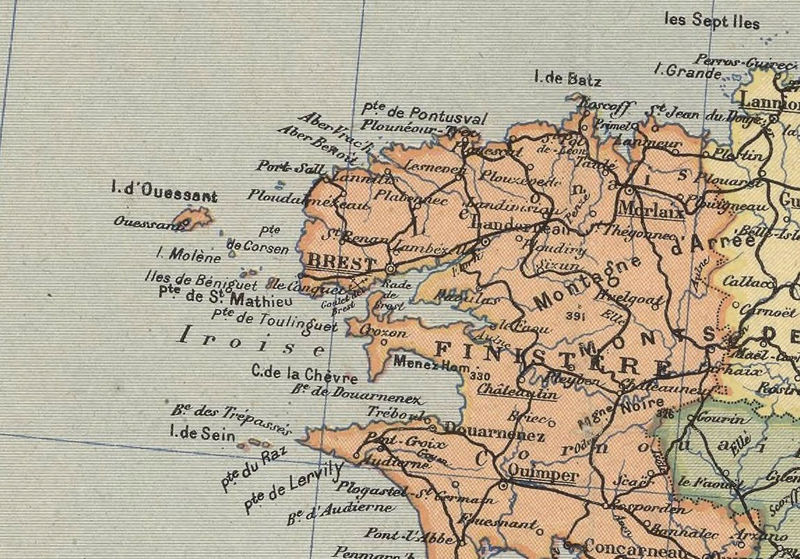
\includegraphics[width = \linewidth, outer]{figures/bretagne.png}
% \end{figure}


To put a graphics in the text like in the figure \ref{fig:figure-text}, use\sidenote{The \texttt{\textbackslash label} \textit{has} to be inside the \texttt{\textbackslash sidecaption} command, otherwise references with \texttt{\textbackslash ref} won't work.}

\begin{codebox}{tex}
\begin{figure}
	\sidecaption{<caption>\label{<label>}} % put this on top
	% \label HAS to be inside the \sidecaption
	\includegraphics[]{<>} % or tikz or anything
\end{figure}
\end{codebox}


To put a figure in the margin like the figure \ref{fig:figure-margin}, use

\begin{codebox}{tex}
\begin{marginfigure}
	\includegraphics[]{<>} % or tikz or anything
	\caption{<caption>\label{<label>}}
\end{figure}
\end{codebox}

\marginfig{figures/marine-knots.jpg}{The most common sea boat knots. This image can be displayed rather small, so it fits in the margin. The caption is displayed below.}{fig:figure-margin}

For wide figures like the figure \ref{fig:figure-fullwidth}, use

\begin{codebox}{tex}
\begin{figure*}
	\includegraphics[]{<>} % or tikz or anything
	\sidecaption{<caption>\label{<label>}}
\end{figure*}
\end{codebox}

\newpage

\widefig{figures/usa-census.png}{The US census map from data collected in 2010 -- \url{www.ecpmlangues.u-strasbg.fr}\\This is a wide figure, stretching from the innermost to the outermost margin.}{fig:figure-fullwidth}


\subsection{Shortcuts}

I find typing figure environments repetitive for long (even short) documents, so I made the following macro for figures with \texttt{\textbackslash sidecaption}s :

\begin{codebox}{tex}
\textfig[<optional width>]{<file path>}{<caption>}{<label>}
\end{codebox}

The \inlinecode{}{<optional width>} is a number between zero and one wich determines the image width relative to the text width. The default value is 1, like on the figure \ref{fig:figure-text}.

The same macros are provided for images in the magins and wide images, respectively shown in figures \ref{fig:figure-margin} and \ref{fig:figure-fullwidth}.

\begin{codebox}{tex}
% figure in the margin
\marginfig[<optional width>]{<file path>}{<caption>}{<label>}
% wide figure
\widefig[<optional width>]{<file path>}{<caption>}{<label>}
\end{codebox}



If for any reason a figure caption has to be put in the main text block, just use the regular \texttt{figure} environment. The following shortcut macros will also do. The result of \inlinecode{tex}{\plainfig} is shown in figure \ref{fig:figure-plain}.

\begin{codebox}{tex}
% plain figure with textwidth
\plainfig[<optional width>]{<file path>}{<caption>}{<label>}
% plain figure with full width
\plainwidefig[<optional width>]{<file path>}{<caption>}{<label>}
\end{codebox}

% \plainfig[.7]{figures/mandelbrot.png}{The Mandelbrot set with different depths of iteration. This caption is not in the margin but in the main text area. It can sometimes be useful with really really long captions. \lipsum[1]}{fig:figure-plain}

\begin{figure}[htb!]
    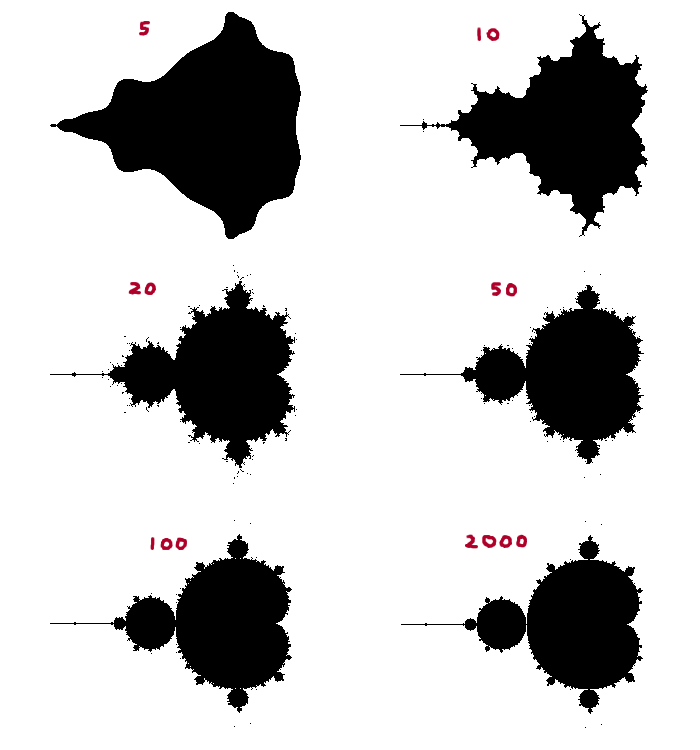
\includegraphics[width =.7\linewidth]{figures/mandelbrot.png}
    \caption[The Mandelbrot set with different depths of iteration. This caption is not in the margin but in the main text area. It can sometimes be useful with really really long captions.]{The Mandelbrot set with different depths of iteration. This caption is not in the margin but in the main text area. It can sometimes be useful with really really long captions. \lipsum[1]\label{fig:figure-plain}}

\end{figure}

\newpage

\subsection{Tables}

Table environments work the same as figures, as is is shown in tables \ref{tab:table-text} and \ref{tab:table-wide}.

\begin{table}[!htb]\small
\sidecaption{The elementary particles included in the standard model. This is a table with a \texttt{\textbackslash sidecaption}.\label{tab:table-text}}
\begin{tabular}{lllll}
	\multicolumn{5}{l}{\textbf{The Standard model of Elementary Particles.}}\\
	\toprule
	\multicolumn{3}{l}{\textbf{Three generations of matter (fermions)}} & \multicolumn{2}{l}{\textbf{Interactions (bosons)}} \\
	I & II & III & & \\
	% \cmidrule(lr){1-3}\cmidrule(lr){4-5}
	\multicolumn{3}{c}{\textsc{quarks}} & \textsc{gauge} & \textsc{scalar} \\
	\cmidrule(lr){1-3}\cmidrule(lr){4-4}\cmidrule(lr){5-5}
	\textbf{u}~~up & \textbf{c}~~charm & \textbf{t}~~top & \textbf{g}~~gluon & \textbf{H}~~higgs \\
	\textbf{d}~~down & \textbf{s}~~strange & \textbf{b}~~bottom & \textbf{\textgamma}~~photon & \\
	\multicolumn{3}{c}{\textsc{leptons}} & \textbf{Z} boson  & \\
	\cmidrule(lr){1-3}
	\textbf{e}~~electron & \textbf{\textmu}~~muon & \textbf{\texttau}~~tau & \textbf{W} boson & \\
	\textbf{\textnu\textsubscript{e}}~~el. neutrino & \textbf{\textnu\textsubscript{\textmu}}~~mu. neutrino & \textbf{\textnu\textsubscript{\texttau}}~~tau neutrino &  & \\
	\bottomrule
\end{tabular}
\end{table}


% \begin{table*}[!htb]\small
% \begin{tabularx}{\linewidth}{rXXXXXXrXXXXXX}
% 	\multicolumn{14}{l}{\textbf{Table des marées au port de Douarnenez (Finistère).}} \\
% 	\toprule
% 	 & \multicolumn{3}{c}{\textbf{Ven. 23 juillet 2021}} & \multicolumn{3}{c}{\textbf{Sam. 24 juillet 2021}} & & \multicolumn{3}{c}{\textbf{Dim. 25 juillet 2021}} & \multicolumn{3}{c}{\textbf{Lun. 26 juillet 2021}} \\
% 	 & heure & hauteur & coef. & heure & hauteur & coef. & & heure & hauteur & coef. & heure & hauteur & coef. \\
% 	\cmidrule(lr){2-4}\cmidrule(lr){5-7}\cmidrule(lr){9-11}\cmidrule(lr){12-14}
% 	\textsc{bm} & 04:54 & 6.06 & 81 & 05:46 & 6.24 & 88 & \textsc{pm} & 00:21 & 0.92 & -- & 01:08 & 0.88 & -- \\
% 	\textsc{pm} & 11:05 & 1.38 & -- & 11:55 & 1.19 & -- & \textsc{bm} & 06:34 & 6.34 & 92 & 07:19 & 6.33 & 92 \\
% 	\textsc{bm} & 17:17 & 6.39 & 85 & 18:06 & 6.59 & 91 & \textsc{pm} & 12:41 & 1.10 & -- & 13:26 & 1.12 & -- \\
% 	\textsc{pm} & 23:33 & 1.10 & -- & ---:--- & -- & -- & \textsc{bm} & 18:52 & 6.67 & 93 & 19:36 & 6.63 & 91 \\
% 	\bottomrule
% \end{tabularx}
% \sidecaption{Table des marées à Douarnenez du 23 au 26 juillet 2021, Service Hydrographique et Océanographique de la Marine, \url{maree.shom.fr}.\\This is a wide table, called with the \inlinecode{tex}{table*} environment. The caption is also a \inlinecode{tex}{\sidecaption{}}.\label{tab:table-wide}}
% \end{table*}Improper alphabetic constant.


% To typeset the table \ref{tab:table-text}, use the following code, which is just a \inlinecode{tex}{table} environment with a \inlinecode{tex}{\sidecaption}. For table \ref{tab:table-wide}, use the \inlinecode{tex}{table*} environment with either \inlinecode{tex}{\sidecaption} or \inlinecode{tex}{\caption}.\inlinecode{tex}{\FloatBarrier} is there to make sure the floats appear in order.\sidenote[][100pt]{\inlinecode{tex}{\FloatBarrier} works for all floating environments, including figures.}

\begin{codebox}{tex}
\begin{table}[!htb]\small
	\sidecaption{The elementary particles included in the standard model. This is a table with a \texttt{\textbackslash sidecaption}.\label{tab:table-text}}
	\begin{tabular}{lllll}
		\multicolumn{5}{l}{\textbf{The Standard model of Elementary Particles.}}\\
		\toprule
		\multicolumn{3}{l}{\textbf{Three generations of matter (fermions)}} & \multicolumn{2}{l}{\textbf{Interactions (bosons)}} \\
		I & II & III & & \\
		\multicolumn{3}{c}{\textsc{quarks}} & \textsc{gauge} & \textsc{scalar} \\
		\cmidrule(lr){1-3}\cmidrule(lr){4-4}\cmidrule(lr){5-5}
		\textbf{u}~~up & \textbf{c}~~charm & \textbf{t}~~top & \textbf{g}~~gluon & \textbf{H}~~higgs \\
		\textbf{d}~~down & \textbf{s}~~strange & \textbf{b}~~bottom & \textbf{\textgamma}~~photon & \\
		\multicolumn{3}{c}{\textsc{leptons}} & \textbf{Z} boson  & \\
		\cmidrule(lr){1-3}
		\textbf{e}~~electron & \textbf{\textmu}~~muon & \textbf{\texttau}~~tau & \textbf{W} boson & \\
		\textbf{\textnu\textsubscript{e}}~~el. neutrino & \textbf{\textnu\textsubscript{\textmu}}~~mu. neutrino & \textbf{\textnu\textsubscript{\texttau}}~~tau neutrino &  & \\
		\bottomrule
	\end{tabular}
\end{table}
\end{codebox}

% \begin{codebox}{tex}
% \begin{table*}[!htb]\small
% 	\begin{tabularx}{\linewidth}{rXXXXXXrXXXXXX}
% 		\multicolumn{14}{l}{\textbf{Table des marées au port de Douarnenez (Finistère).}} \\
% 		\toprule
% 			& \multicolumn{3}{c}{\textbf{Ven. 23 juillet 2021}} & \multicolumn{3}{c}{\textbf{Sam. 24 juillet 2021}} & & \multicolumn{3}{c}{\textbf{Dim. 25 juillet 2021}} & \multicolumn{3}{c}{\textbf{Lun. 26 juillet 2021}} \\
% 			& heure & hauteur & coef. & heure & hauteur & coef. & & heure & hauteur & coef. & heure & hauteur & coef. \\
% 		\cmidrule(lr){2-4}\cmidrule(lr){5-7}\cmidrule(lr){9-11}\cmidrule(lr){12-14}
% 		\textsc{bm} & 04:54 & 6.06 & 81 & 05:46 & 6.24 & 88 & \textsc{pm} & 00:21 & 0.92 & -- & 01:08 & 0.88 & -- \\
% 		\textsc{pm} & 11:05 & 1.38 & -- & 11:55 & 1.19 & -- & \textsc{bm} & 06:34 & 6.34 & 92 & 07:19 & 6.33 & 92 \\
% 		\textsc{bm} & 17:17 & 6.39 & 85 & 18:06 & 6.59 & 91 & \textsc{pm} & 12:41 & 1.10 & -- & 13:26 & 1.12 & -- \\
% 		\textsc{pm} & 23:33 & 1.10 & -- & ---:--- & -- & -- & \textsc{bm} & 18:52 & 6.67 & 93 & 19:36 & 6.63 & 91 \\
% 		\bottomrule
% 	\end{tabularx}
% 	\sidecaption{Table des marées à Douarnenez du 23 au 26 juillet 2021, Service Hydrographique et Océanographique de la Marine, \url{maree.shom.fr}.\\This is a wide table, called with the \inlinecode{tex}{table*} environment. The caption is also a \inlinecode{tex}{\sidecaption{}}.\label{tab:table-wide}}
% \end{table*}\FloatBarrier
% \end{codebox}

To produce tables in the margin like table \ref{tab:table-margin}, use the \inlinecode{tex}{margintable} environment like in the following.

\begin{margintable}[0pt]\small
\caption{Major, minor and perfect music intervals. ST. stands for \textit{semitones}. This table is in the margin. \label{tab:table-margin}}
\begin{tabular}{ll}
	\toprule
	\textbf{ST.} & \textbf{Intervals} \\
	\midrule
	0 & unison \\
	1 & minor second \\
	2 & major second \\
	3 & minor third \\
	4 & major third \\
	5 & perfect fourth \\
	6 & aug. 4\textsuperscript{th} / dim. 5\textsuperscript{th} \\
	7 & perfect fifth \\
	8 & minor sixth \\
	9 & major sixth \\
	10 & minor seventh \\
	11 & major seventh \\
	12 & octave \\
	\bottomrule
\end{tabular}
\end{margintable}

\begin{codebox}{tex}
\begin{margintable}[]\small
	\caption{Major, minor and perfect music intervals. ST. stands for \textit{semitones}. This table is in the margin. \label{tab:table-margin}}
	\begin{tabular}{ll}
		\toprule
		\textbf{ST.} & \textbf{Intervals} \\
		\midrule
		0 & unison \\
		1 & minor second \\
		2 & major second \\
		3 & minor third \\
		4 & major third \\
		5 & perfect fourth \\
		6 & aug. 4\textsuperscript{th} / dim. 5\textsuperscript{th} \\
		7 & perfect fifth \\
		8 & minor sixth \\
		9 & major sixth \\
		10 & minor seventh \\
		11 & major seventh \\
		12 & octave \\
		\bottomrule
	\end{tabular}
\end{margintable}
\end{codebox}

\newpage

\subsection{Code}
\label{sub:code}

Code can be inserted, whether with simple code boxes or captioned snippets that look like the following.
\begin{snippet}{c}{Hello world in C. This is a captioned code snippet.}{snp:hello-world}
int main(int argc, char *argv[]) {
	printf("Hello world!");
	return 0;
}
\end{snippet}

The box is a light gray hairline that helps make the code stick out just enough without distracting the eye too much. The code itself is syntax colored according to the used language. There are several environments for code boxes, explained below.

For a simple code box with neither line numbering nor caption, the macro environment is the following.

\sidetext{%
This supports most of the classic languages. Here are some examples for the language option:

\inlinecode{}{c},

\indent\inlinecode{}{c++},

\indent\inlinecode{}{python},

\indent\inlinecode{}{java},

\indent\inlinecode{}{latex}\dots\\
If a specific language is not recognized, use the \inlinecode{}{text} option instead: it will display the code without syntax coloring.
}%
% \begin{altcodebox}{tex}
% \begin{codebox}{<your language in lowercase>}
% <
% Your code. It can contain all special characters such as { } ( ) [ ] \ % (the percent mark here is grayed just because on this very code box the language is set on latex)
% It break lines.
% It will end only when reading the %\end{codebox} below.
% >
% \end{codebox}
% \end{altcodebox}

For a code box \textit{with} line numbering --still without a caption-- use the following environment.
% \begin{altcodebox}{tex}
% \begin{codeboxnum}{<your language in lowercase>}
% <your code>
% \end{codeboxnum}
% \end{altcodebox}

For captioned code snippets, the same environments exist, as shown as follows. For example, the listings \ref{snp:hello-world} and \ref{snp:snowflakeos} are respectively unnumbered and numbered code snippets.

\begin{codebox}{tex}
\begin{snippet}{<language>}{<caption>}{<label>}
This code will be displayed in a captioned code box, without line numbering.
\end{snippet}

\begin{snippetnum}{<language>}{<caption>}{<label>}
This code will be displayed in a captioned code box, with line numbering.
\end{snippetnum}
\end{codebox}

Small pieces of code can be useful to put in flow of the text. This class provides a command to things like this: \inlinecode{c++}_public int size() {}_. Use the following to insert a piece of code in the text.


% \sidetext{If the piece of code inside the \inlinecode{tex}{\inlinecode} contains curly braces, use another character to delimit your code, the same at beginning and end. Underscore (\texttt{\char`_}) and pipe (\texttt{|}) will do fine.}
% \begin{codebox}{tex}
% \inlinecode{<language>}{<your code>}
% % if there are curly braces in your code
% \inlinecode{<language>}_<your code>_ % or
% \inlinecode{<language>}|<your code>|
% \end{codebox}

\inlinecode{tex}{\inlinecode} does not break at lines, so be careful, it can sometimes protrude on the right margin. If it is the case, go to a new line by inserting \inlinecode{tex}{\\} just before \inlinecode{tex}{\inlinecode}.


The following chunk is an example snippet to show the look when the code is a bit heftier. See how the box breaks at the end of the page.

\begin{snippetnum}{c}{A source code snippet of \texttt{29jm}'s stunningly amazing \href{https://github.com/29jm/SnowflakeOS}{\texttt{SnowflakeOS}}. This is a numbered code snippet that goes through several pages.}{snp:snowflakeos}
#include <kernel/multiboot2.h>
#include <kernel/sys.h>

static const char* tag_table[] = {
	"TAG_END",
	"TAG_CMDLINE",
	"<unknown>",
	"TAG_MODULE",
	"TAG_MEM",
	"TAG_BOOTDEV",
	"TAG_MEMMAP",
	"TAG_VBE",
	"TAG_FB",
	"<unknown>",
	"TAG_APM",
	"<unknown>",
	"<unknown>",
	"<unknown>",
	"TAG_RSDP1",
	"TAG_RSDP2",
};

/* Prints the multiboot2 tags given by the bootloader.
*/
void mb2_print_tags(mb2_t* boot) {
	if (boot->total_size <= sizeof(mb2_t)) {
		printke("no tags given");
		return;
	}

	mb2_tag_t* tag = boot->tags;
	mb2_tag_t* prev_tag = tag;

	do {
		const char* tag_name;

		if (tag->type < sizeof(tag_table) / sizeof(tag_table[0])) {
			tag_name = tag_table[tag->type];
		} else {
			tag_name = "<unknown>";
		}

		printk("%12s (%2d): %d bytes", tag_name, tag->type, tag->size);

		prev_tag = tag;
		tag = (mb2_tag_t*) ((uintptr_t) tag + align_to(tag->size, 8));
	} while (prev_tag->type != MB2_TAG_END);
}

/* Returns the first multiboot2 tag of the requested type.
*/
mb2_tag_t* mb2_find_tag(mb2_t* boot, uint32_t tag_type) {
	mb2_tag_t* tag = boot->tags;
	mb2_tag_t* prev_tag = tag;

	do {
		if (tag->type == tag_type) {
			return tag;
		}

		prev_tag = tag;
		tag = (mb2_tag_t*) ((uintptr_t) tag + align_to(tag->size, 8));
	} while (prev_tag->type != MB2_TAG_END);

	return NULL;
}
\end{snippetnum}


\section{The titlepage}

\section{Compilation}



\part*{Appendix}
\appendix

\chapter[Some additional stuff]{Some additional stuff (see how the title protrudes in the margin)}

\lipsum \cite{BringhurstEoTS}



\loadgeometry{evenmargins}

\backmatter

\printbibliography
\printindex

\end{document}